



\subsection{System Architecture Overview}
\label{sec:overview}

Our architecture can be separated into three parts:

\begin{enumerate}
\item Speech to Text Conversion: Using the AMI and ICSI corpus, we transcribed the audio files using Whisper. Next, we diarized the audio file using Pyannote and combined the two files into a single transcription.

\item Text Summarization: Using the human reference and the dataset that we have created we combined both to form a single JSON file. We then fed the JSON file into the pretrained BART model.

\item User Interface: Using the Django Framework, we created a simple web application that allows users to upload an audio file and receive a transcription and a summary of the meeting.
\end{enumerate}

The proposed pipeline is implemented in Python 3.8 using various tools. A complete list of tools we used as follows: BART \textcolor{red}{[open source code cite?]}, FFMEG \cite{FFmpeg}, Whisper Open AI \cite{whisper}, Pyannote \cite{pyannotewhisper}, Hugging Face Transformers \textcolor{red}{[open source code cite?]}, and Django \cite{Django} . 

%\cite{whisper, } are used with speaker diarization where the audio is partitioned into segments to identify speakers.  




\subsection{Speech to Text Conversion}
\label{sec:stc}
\textcolor{red}{Need to explain the methods for speech to text conversion}




\subsection{Text Summarization}
\label{sec:ts}

\subsubsection{BART}


Our pretrained model is BART (Bidirectional Auto-Regressively Transformer). BART was developed by Facebook AI Research team. BART can handle various NLP tasks, for example, translation, text classification, summarization, etc. BART can be fine-tuned for any text generation and comprehension tasks. In short, BART is pretrained by corrupting the input text using some noise schemes and learning a model to reconstruct the original input.


%\begin{figure}[thpb]
%\centering
%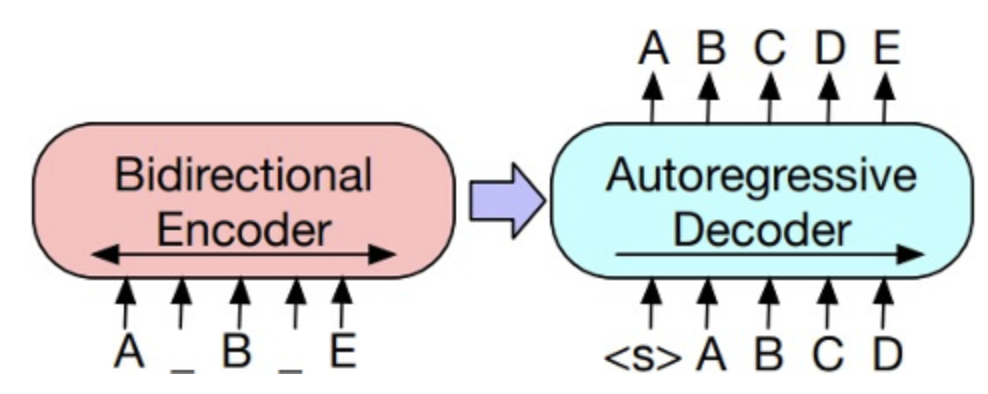
\includegraphics[width=7cm, height=2.5cm]{figures/BART}
%\caption{Encoder decoder model}
%%\Description{autoencoder}
%\label{fig:TL}
%\textcolor{red}{Notes: the figure will be replaced with a new figure}
%\end{figure}


BART has three big components: 1) noise transformation, 2) bidirectional encoder, and 3) autoregressive decoder.
i.	Noise transformation happens right before the encoder. Noise transformation will add some noises onto the inputs before feeding the data into the encoder. Having such action is to prevent the overfitting problem. There are five ways of corrupting the input: Token Masking, Sentence Permutation, Document Rotation, Token Deletion, and Text Infilling. The authors examined all of them and found that BART with text infilling could give the most consistently strong performance.
ii.	Next, the corrupted data will feed into the encoder that is able to read in both directions. This encoder produces a set of hidden states that capture the meaning and context of the input text.
iii.	Lastly, the set of hidden states will then get pushed to the autoregressive decoder that reads from left to right. This decoder basically generates a probability distribution over all possible tokens, given the hidden states and the masked input text. It then samples a token from the distribution and appends it to the output text in a step-by-step manner, where each token is conditioned on the previously generated tokens.

One reason why we choose BART is that it has richer documentation on how users can do fine- tuning and feed their own dataset to suit their own needs, compared to other novel pretrained models. Also, BART can establish abstractive summarization which is our objective. The evidence shown in the paper is highly abstractive with only a few phrases copied from the input.



\subsubsection{Transfer Learning in BART}
As mentioned above, BART hasn’t been trained on any long conversation dataset that includes multiple speakers. We plan to feed some of the AMI and ICIS corpus to BART and utilize another portion of the data to validate the outcome.

We are using transfer learning to train our model. In transfer Learning we need select a baseline model which acts as the source model, and we fine-tuned using the dataset. For each of the experiments we evaluated the experiment outcomes using both qualitative and quantitative metrics which are discussed in the nest section.

For faster prototyping, we used the HuggingFace Trainer API which allows us to use train models and save the best. The Trainer API also allows us to use TensorBoard to evaluate the training and evaluation performances. Once uploaded to HuggingFace, we can utilize the instant Inference API to use our model for demos.


\begin{figure}[thpb]
	\centering
	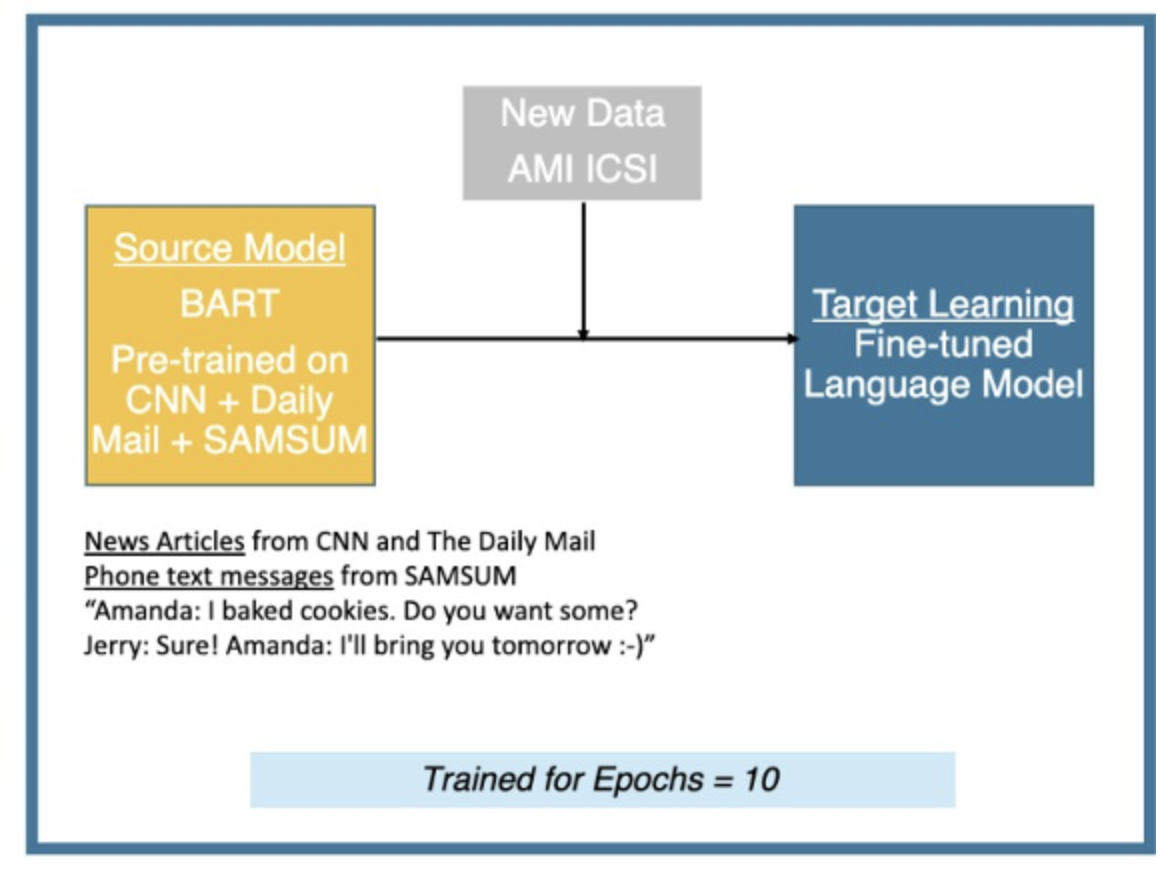
\includegraphics[width=7cm, height=4.5cm]{figures/TL}
	\caption{Transfer learning model}
	%\Description{autoencoder}
	\label{fig:TL}
	\textcolor{red}{Notes: the figure will be replaced with a new TL}
\end{figure}


\subsection{User Interface}
The application consists of two pages, with the first page dedicated to transcription and the second to summarization. Starting with the first page, at the top of our user interface, we offer the browse and upload buttons for users to locate and upload their local files. A clear button is also provided to reset the current application state to the initial state, enhancing visibility.

Beneath these buttons, we offer a transcription box that contains the transcribed content from the audio file. The transcription box enables users to edit the transcribed content if they find it necessary to change a word, number, or sentence. The reason for providing such editing functionality is that the accuracy of converting audio to text heavily depends on the quality of the microphone input.

Currently, our system is unable to identify speaker names mentioned in any conversation for accurate speaker labeling. Therefore, below the transcription box, we provide a table with the first column displaying the speaker tags identified by our system, and the second column allowing users to change the corresponding speaker tags to names of their choice. To apply all changes made, a change button is provided next to the table. We also provide a download link that allows users to download the updated transcript if they wish to save it locally.

At the bottom of our user interface, we incorporate an audio player and display an unmodifiable original content box, allowing users to listen and track the progress. Users can hover over and click on any point in the timeline, and the audio player will automatically jump to the selected time.

Navigating to the second page of our application, users can read the summary of the updated transcript. To obtain the system-generated summary, users must click the "Get my summary" button to initiate the summarization process. After a certain amount of processing time, the summary will appear in the box located below the button. Lastly, keywords from the meeting are also provided. These keywords are extracted from the transcription box on the first page. Arranged from top to bottom, the first list contains single words, the second list contains pairs of words, and the third list contains groups of three consecutive words. These keywords are offered to help users better comprehend the conversation.

\textcolor{red}{Need to explain the methods for user interface \& figures???. its above in black }

\vspace{15mm}




%
%\begin{algorithm}[tphb]
%%	\setstretch{1.6}
%	\caption{ANVO($D_{train}$, $k_{min}$, $k_{max}$, $\epsilon$)} \label{alg:sampling1}
%	\begin{algorithmic}[1]
%		\STATE \textbf{Input: } 
%	$D_{train}$ is a set of number of class-labeled training data points, $k_{min}$ is the minimum $k$ value for  $KNN$ search, $k_{max}$ is the maximum $k$ value, $\epsilon$ is the value to add to each attribute of the generated data point if the average difference is equal to the zero vector.  \\
%		\STATE \textbf{Output:} A balanced training dataset augmented by synthetic data\\ 
%		\STATE \textbf{Method:}
%		\STATE Split $D_{train}$  into majority class dataset ($MA$) and minority class dataset ($MI$) and record their number of instances as $N_{MA}$ and $N_{MI}$, respectively.  
%		\STATE $N_{syn} \leftarrow N_{MA} - N_{MI}$
%		\IF{If $k_{max} > N_{MI}-1$} \STATE $k_{max} \leftarrow N_{MI}-1$
%		\ENDIF
%		\IF{If $k_{min} \geq k_{max}$} \STATE $k_{min} \leftarrow \lceil\frac{k_{max}}{2}\rceil$
%		\ENDIF
%		\STATE Initailization: $S \leftarrow \{\}$, $i \leftarrow 1$, $\overrightarrow{avg_{diff}} \leftarrow $ 0 for all attributes in $D_{train}$, $\overrightarrow{avg_{diff}}$ is the average vector of the differences between the selected minority data point and its $k$ neighbors
%		\REPEAT
%			\STATE $P \leftarrow $ Choose a random minority data point %that has not already used all the possible $k$ values to generate data, save as point
%			\STATE $k \leftarrow $ Choose a random integer in the range $[k_{min}, k_{max}]$ that has not already been used with the point $P$ to generate data
%			\STATE Find the $k$ nearest neighbors of $P$ using $MI$ as the search space
%			\STATE $\overrightarrow{avg_{diff}} \leftarrow $ obtain a vector that represents the average difference between $P$ and its $k$ neighbors. 
%			\STATE $P_{new} \leftarrow $ Generate a new data point, $P_{new} = P + \overrightarrow{avg_{diff}}$
%			\IF{$\overrightarrow{avg_{diff}} = \vec{0}$}
%				\STATE $P_{new} \leftarrow = P + \overrightarrow{\epsilon}$ 
%			\ENDIF
%			\STATE $S \leftarrow$ add ${\P_{new}}$
%		\UNTIL{$i \leq N_{syn}$, If there are still possible data points left to generate (i.e., all the minority points have not used all the possible $k$ values to  generate data)
%		}
%	    \STATE $D_{train} \leftarrow D_{train} + S$
%	    \STATE return $D_{train}$, this is a balanced training data augmented by minority class synthetic data
%	\end{algorithmic}
%\end{algorithm}





%\begin{center}
%	\begin{figure*}
%		%	\widefigure
%		\begin{center}
%			\begin{subfigure}{0.35\textwidth}
%				\includegraphics[width=7.6cm, height=4.65cm]{figures-quan/LR1}
%				\caption{LR}
%				\label{fig:first}
%			\end{subfigure}  
%			\hspace{20mm}
%			\begin{subfigure}{0.35\textwidth}
%				\includegraphics[width=7.6cm, height=4.65cm]{figures-quan/LR2}
%				\caption{NN-based TL + LR}
%				\label{fig:second} 
%			\end{subfigure} \\
%			\vspace{5mm}
%			\caption{Model performance summary of 19 individuals: LR vs. NN-based TL + LR}
%			\label{fig:TLLR} 
%		\end{center}
%	\end{figure*}
%\end{center}
%
%

%\begin{equation}
%	\label{eq:eq1}
%	Exposure(x_i, t) = \sum_{j=1}^{N}E_i * t_{j, i}:
%\end{equation}
%
%math equation example in \ref{eq:eq2}. 
%
%\begin{math}
%	\label{eq:eq2}
%	\pi^{'}(\theta) = \pi(\theta|D)
%\end{math}
%by Bayes' formula.
%
%More examples are in \ref{eq:eq3}. 
%
%\begin{eqnarray}\label{hyper-update}
%	V_i^* & = &\frac{V_i}{1+c_iV_i} \label{eq:eq4}\\
%	m_i^* &= &\left(\frac{m_i}{V_i}+c_i\overline{t_i}\right)\frac{V_i}{1+c_iV_i} \label{eq:eq5}\\
%	% m_i^* &= &\left(\frac{m_i}{V_i}+c_i\overline{t_i}\right)V_i^*\\
%	a_i^* &= &a_i + \frac{c_i}{2}  \label{eq:eq6} \\
%	b_i^* &= &b_i + \frac12\left[\frac{m_i^2}{V_i}+\left(\sum_{r = 1}^{c_i}t_{i,r}^2\right)-\frac{{m_i^*}^{2}}{V_i^*}\right]  \label{eq:eq3}
%\end{eqnarray}






